\section{Analyse et Conception}


Pour faire face à la complexité croissante des systèmes d’informations, de
nouvelles méthodes et outils ont été créés.Dans le cadre de notre analyse,
c’est un langage appelé UML (Unified Modeling Language) qui est celui retenu pour la modélisation du système à mettre en place.

En effet l'UML se traduit par un Langage de modélisation unifié. Il s’agit d’un langage visuel constitué d’un ensemble de schémas, appelés diagrammes, donnant chacun une vision différente du système à traiter. L'UML nous fournit donc des diagrammes pour représenter l’application à développer: son fonctionnement, sa mise en route, les actions susceptibles d’être effectuées par l’application, etc. L'UML, est un langage basé sur le concept de la Programmation Orientée Objet. Il ne préconise aucune démarche, ce n’est donc en aucun cas une méthode. Chacun est libre d’utiliser les types de diagramme qu’il souhaite, dans l’ordre qu’il veut. Il suffit que les diagrammes réalisés soient cohérents entre eux, avant de passer à la réalisation de l’application.


\subsection{Étude des Processus Métier}
Les processus métier constituent le mécanisme principal par lequel les services d'entreprise sont intégrés. C'est un ensemble d'activité visant à atteindre un objectif particulier d'une entreprise. Ce processus métier apporte une vision du métier réel, et constitue un excellent instrument de formalisation et d'analyse dans la construction des systèmes.
Dans le cas d'Oqenyite, les processus métier sont les suivants créer boutique, gérer catalogue en ligne, effectuer commande.
 

\subsubsection* {Gérer boutique}
Le processus gérer un boutique consiste à  
modifier les différents produits de la boutique: ajouter supprimer classer les produits par catégorie.  Après ça, il a la possibilité d’exposer ces produits, de donner ces caractéristiques et afficher les prix selon la catégorie de chaque produit. 

\subsubsection*{Gérer catalogue}

Ici le vendeur expose ces produits par catégorie en précisant les caractéristiques suivi des détails tout en mentionnant le prix de chaque produits, les mets en ligne.


\subsubsection*{Effectuer commande}

Pour faire des achats ou pour passer une commande le visiteur ou l'acheteur avant de voir les produit disponible sur la plate-forme d'oqenyite doit se connecter c'est à dire avoir un compte. Une fois connecté l'acheteur a la possibilité de consulter tous les produit existant sur la plate forme, voir leurs caractéristique, ainsi que le prix de chaque produits. Maintenant il fait le choix des produits désirés les ajoutent au panier et passe sa commande.



\subsubsection*{Gérer livraison}

La gestion de la livraison se fait comme suit, l'acheteur après avoir validation du panier choisir son adresse de livraison, si il n'a pas adresse de livraison, il a la possibilité d'ajouter son adresse. Il choisit ensuite le mode de livraison entre livraison (express ou classique). Il sélectionne un moyen de paiement et effectue le paiement.

Le processus métier nous conduit à la réalisation des digrammes d'activités et d'objet de flux.



\subsection{Diagramme d'Activité et Objet de Flux}

Le diagramme d’activité est attaché à une catégorie de classe et décrit le déroulement des activités de cette catégorie. Il indique la part prise par chaque objet dans
l’exécution d’un travail.

Objet de flux est un connecteur avec une pointe de flèche dénotant la direction ou on passe l’objet. Il doit avoir un objet sur au moins une de ses fins. 
Ce diagramme d'activité sera lié au processus effectuer commende.



\begin{minipage}{1\textwidth}
	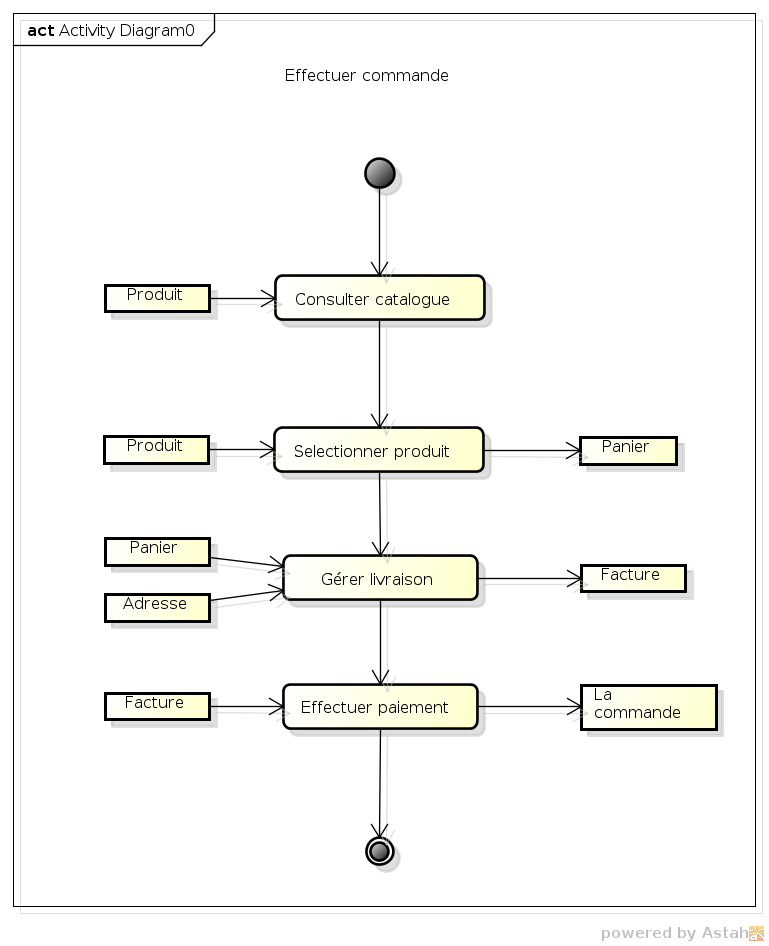
\includegraphics[width=0.7\linewidth]{mama/images/Effectuer}
	\label{fig:Effectuer}
\end{minipage}
\hspace*{\stretch{1}}

Le diagramme d’activité est un Diagramme associé à un objet particulier ou à un ensemble d’objets, qui illustre les flux entre les activités et les actions. Il permet de représenter graphiquement le déroulement d’un cas d’utilisation métier sur les commandes.





\subsection{Cas d'Utilisation Métier}


Le rôle du diagramme de cas d’utilisation métier est de recueillir, d’analyser et d’organiser les besoins, ainsi que de recenser les grandes fonctionnalités d’un système. 

\begin{minipage}{1,1\textwidth}

	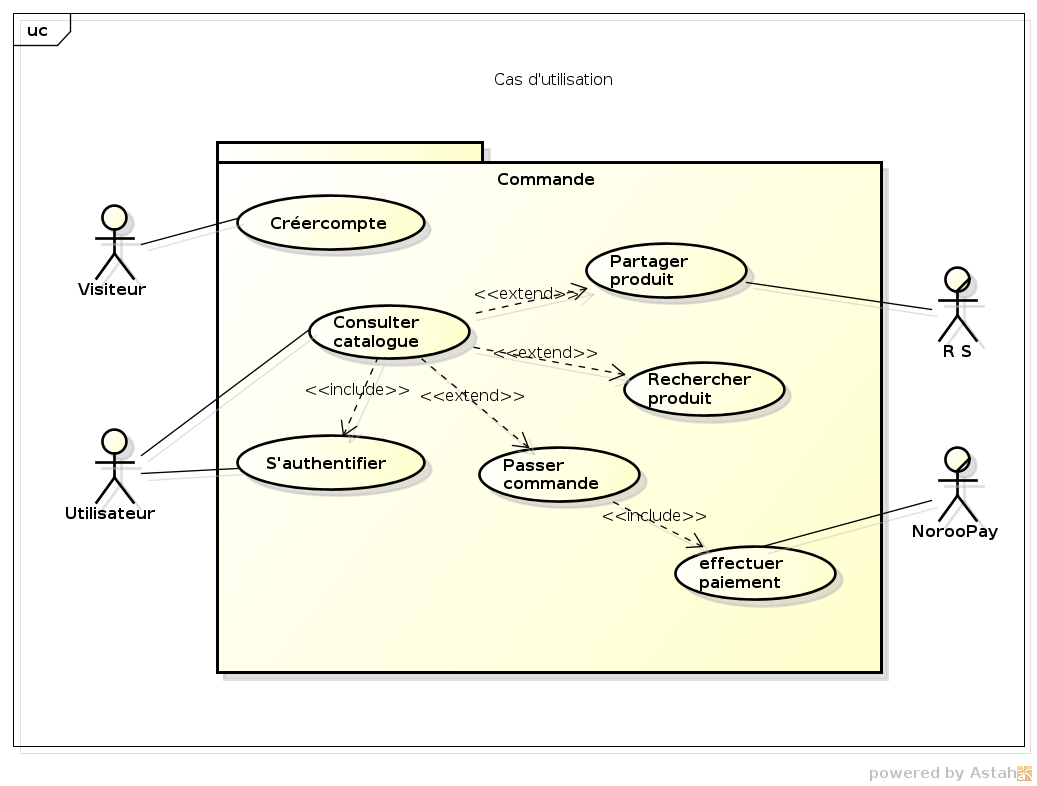
\includegraphics[width=0.7\linewidth]{mama/images/utilisation}
	\label{fig:utilisation}
\end{minipage}
\hspace*{\stretch{1}}



\subsection{Diagramme de Séquence}

le diagramme de séquence est un diagramme d’interaction qui expose en détail
la façon dont les opérations sont effectuées: quels messages sont envoyés et quand ils le sont. Les diagrammes de séquences sont organisés en fonction du temps qui s’écoule au fur et à mesure que nous parcourons la page. Les objets impliqués dans l’opération sont répertoriés de gauche, à droite en fonction du moment où ils prennent part dans la séquence.


%\begin{figure}
%	\centering
%	\includegraphics[width=0.7\linewidth]{mama/images/séquence}
%	\caption{}
%	\label{fig:sequence}
%\end{figure}

\begin{minipage}{0,8\textwidth}
	\includegraphics[width=0.7\linewidth]{mama/images/séquence}
\end{minipage}
\hspace*{\stretch{1}}


\subsection*{Diagramme de classes}

Le diagramme de classes exprime la structure statique du système en termes de classes et de relations entre ces classes. L’intérêt du diagramme de classe est de modéliser les entités du système d’information.
Le diagramme de classe permet de représenter l’ensemble des informations finalisées qui sont gérées par le domaine. Ces informations sont structurées, c’est-à-dire qu’elles sont regroupées dans des classes. Ce
diagramme met en évidence d’éventuelles relations entre ces classes.

\begin{minipage}{1\textwidth}
	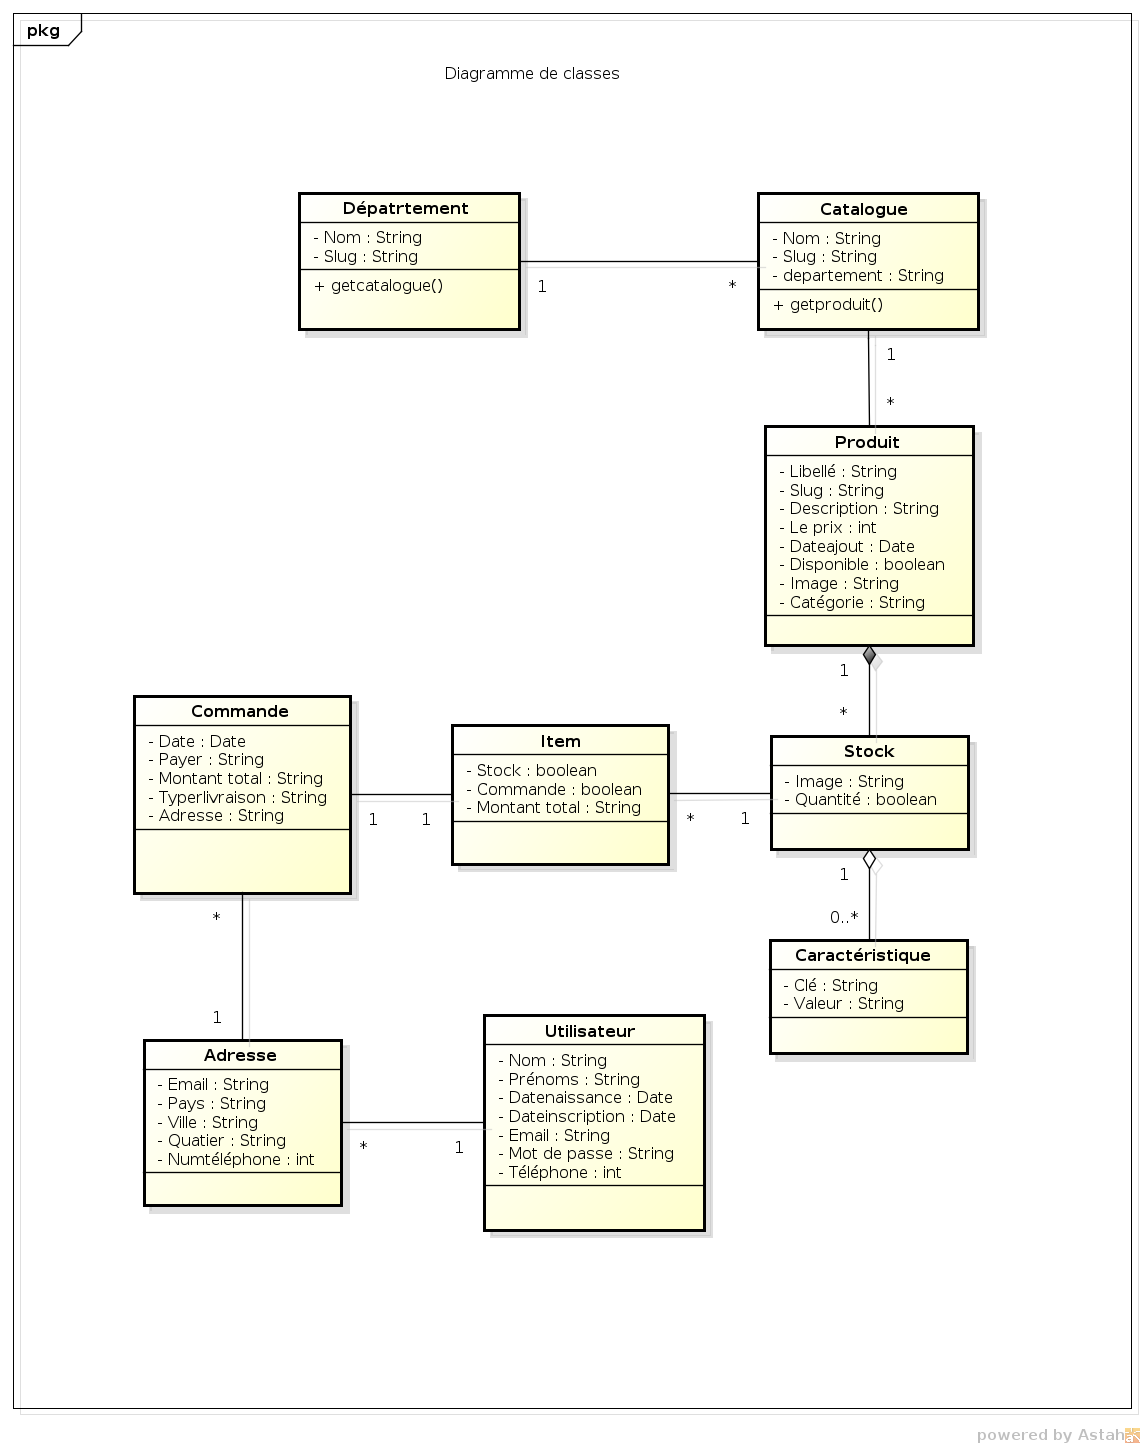
\includegraphics[width=0.7\linewidth]{mama/images/classes}
\end{minipage}
\hspace*{\stretch{1}}


 Chaque classe se décrit par les données et les traitements dont elle est responsable pour elle-même et vis-à-vis des autres classes. Les traitements sont matérialisés par des opérations.


\subsection{Diagramme de Déploiement}

Les diagrammes de déploiement montrent la disposition physique des différents matériels appelés nœuds(ordinateurs, périphériques, réseaux, systèmes de stockage...) qui entrent dans la composition d’un système et la répartition des instances de composants, processus et objets qui vivent sur ces matériels. Les diagrammes de déploiement sont donc très utiles pour modéliser l’architecture physique d’un système.

\begin{minipage}{1,2\textwidth}
	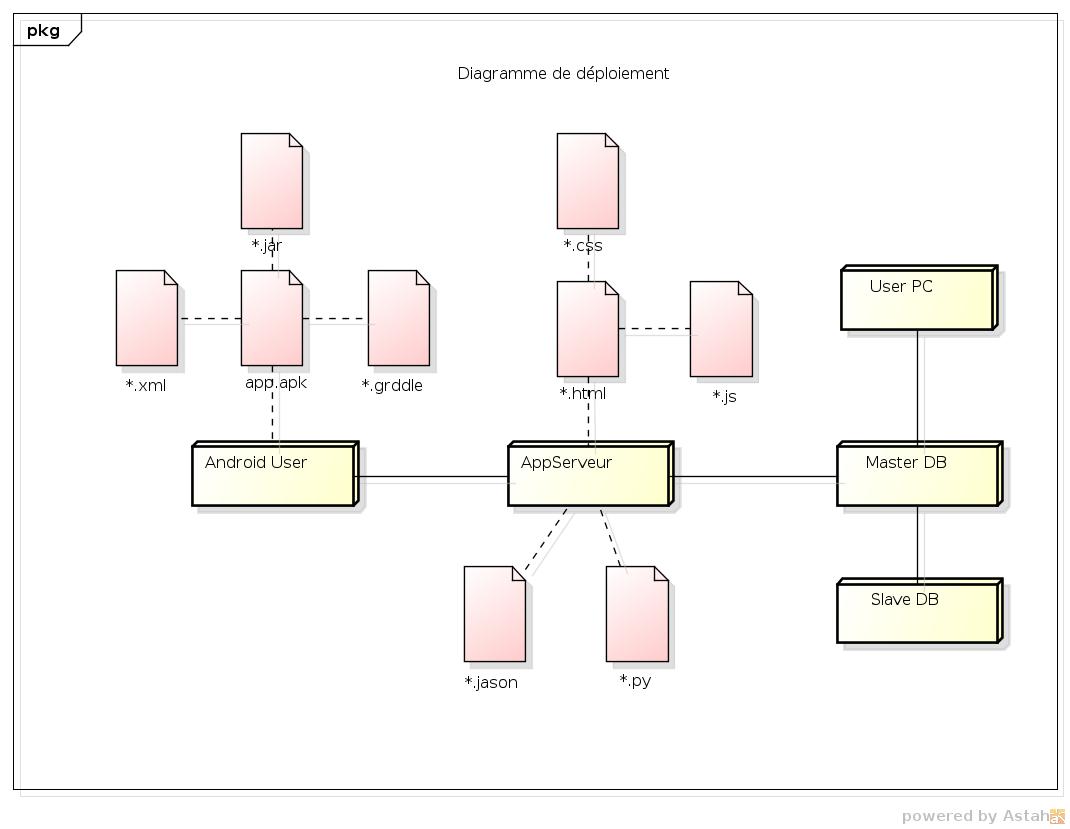
\includegraphics[width=0.7\linewidth]{mama/images/Deployment}
	\label{fig:deployment}
\end{minipage}
\hspace*{\stretch{1}}


 C'est en partant de ces diagrammes qu'on écrit le code informatique pour répondre aux besoins des utilisateurs.



